%initial/final : évolution

Le projet Stibbons a pour but la création d'un environnement de programmation multi-agents pour développeurs de tout niveau. NetLogo (cf. \ref{netlogo-code}) a été un modèle lors de la conception de Stibbons, et une des contraintes alors fixées était d'avoir une application similaire mais exécutant les agents de façon parallèle et non séquencielle comme le fait NetLogo.

\begin{figure}[h]
\centering
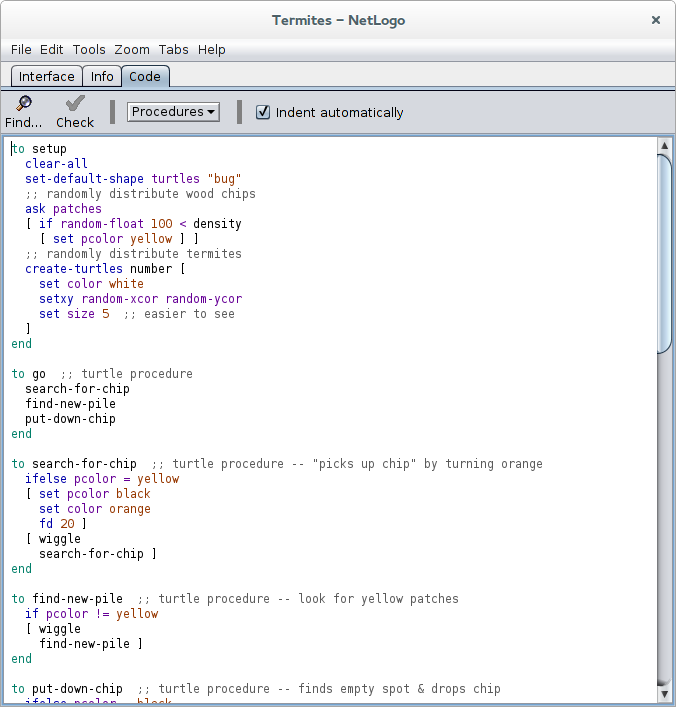
\includegraphics[scale=0.3]{doc/gestionProjet/netlogo-code.png}
\caption{\label{netlogo-code} L'éditeur de texte de NetLogo}
\end{figure}

La finalité d'un tel environnement est de permettre d'effectuer des simulations de comportements d'agents. Un exemple classique est celui dit «~des termites~» (cf. \ref{netlogo-termites}), qui consiste à modéliser des termites ramassant des brindilles pour former leur termitière.
Pour cela, l'utilisateur définit le comportement d'agents représentant ici les termites, étale des brindilles sur le sol, et observe l'agissement de ses agents faire évoluer le modèle.

\begin{figure}[h]
\centering
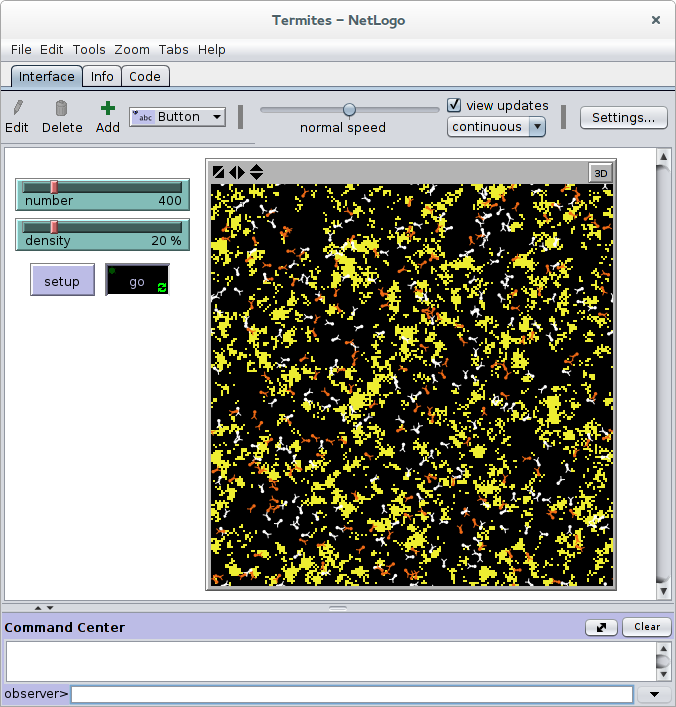
\includegraphics[scale=0.3]{doc/gestionProjet/netlogo-termites.png}
\caption{\label{netlogo-termites} La simulation des termites dans NetLogo}
\end{figure}

Nous avons décidé de créer un langage permettant de manipuler des agents mobiles (dits tortues) afin de les faire se déplacer et communiquer entre eux, soit directement par envoi de messages, soit indirectement en modifiant et analysant leur environnement. Une interface graphique permettant d'observer directement l'évolution du modèle était également prévue.

Au cours du projet, notre encadrant, Michel Meynard, nous a suggéré de permettre l'export du modèle en cours d'exécution (comprenant l'état du monde, des zones le constituant, et des tortues y évoluant), fonctionnalité que nous avons donc rajouté à notre backlog, et à terme à notre application.

Plus tard, il a aussi été décidé de proposer un programme complémentaire à notre application, qui serait utilisable en ligne de commande et ne nécessiterait pas l'utilisation d'un serveur graphique pour fonctionner, mais permettant d'exporter le modèle à intervalle régulier.
Cela permet de ne pas utiliser les ressources graphiques de l'ordinateur, d'exécuter la simulation à pleine vitesse et d'effectuer la simulation sur une ferme de calcul.

Nous avons également décidé d'intégrer un éditeur de texte à l'application principale afin de pouvoir directement éditer et exécuter un programme Stibbons.
